\documentclass{article}
\usepackage{amsmath}
\usepackage{amssymb}
\usepackage{fullpage}
\usepackage{enumerate}
\usepackage{xcolor}
\usepackage{bm}
\pagestyle{empty}
\usepackage{graphicx}
\graphicspath{{C:\Users\Hayden\Desktop\LinAlg\HW9}}
\begin{document}

\noindent{{\Large \bf Fall 25, 4100 Problem Set 9}

\large

\bigskip
\noindent{Please complete all problems. For any proof questions, please structure your proof similar to those from lecture.

\begin{enumerate}

\item Sketch the conic section $x_1^2+8x_1x_2+7x_2^2=1$ by finding the spectral decomposition of the matrix $A=\left[\begin{array}{cc}
1 & 4\\
4 & 7
\end{array}\right]$
\\
\\$x^TAx=1$
\\det $\left[\begin{array}{cc} 1-\lambda & 4 \\ 4 & 7-\lambda \end{array}\right]=(1-\lambda)(7-\lambda)-16=\lambda^2-8\lambda-9=(\lambda-9)(\lambda+1)$
\\$\lambda_1=9$, $\lambda_2=-1$, hyperbola
\\$(A-9I)v_1=\left[\begin{array}{cc} -8 & 4 \\ 4 & -2 \end{array}\right]v_1=0$
\\$v_1=\left[\begin{array}{c} 1 \\ 2 \end{array}\right]$
\\$(A+1I)v_2=\left[\begin{array}{cc} 2 & 4 \\ 4 & 8 \end{array}\right]v_2=0$
\\$v_2=\left[\begin{array}{c} -2 \\ 1 \end{array}\right]$
\\$u_1=\frac{1}{\sqrt{5}}\left[\begin{array}{c} 1 \\ 2 \end{array}\right]$
\\$u_2=\frac{1}{\sqrt{5}}\left[\begin{array}{c} -2 \\ 1 \end{array}\right]$
\\$Q=\left[\begin{array}{cc} u_1 & u_2 \end{array}\right]=\frac{1}{\sqrt{5}}\left[\begin{array}{cc} 1 & -2 \\ 2 & 1 \end{array}\right]$
\\$A=Q\Lambda Q^T$
\\$\Lambda=\left[\begin{array}{cc} 9 & 0 \\ 0 & -1 \end{array}\right]$
\\$y=Q^Tx$, $x^TAx=y^T\Lambda y$
\\$9y_1^2-1y_2^2=1$
\\in $y_1$, $y_2$
\\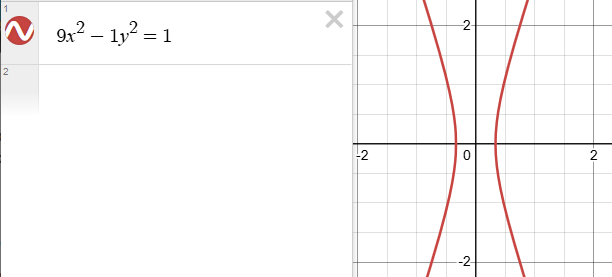
\includegraphics[width=0.8\textwidth]{P11.png}
\\rotated by $Q$ into $x_1$, $x_2$
\\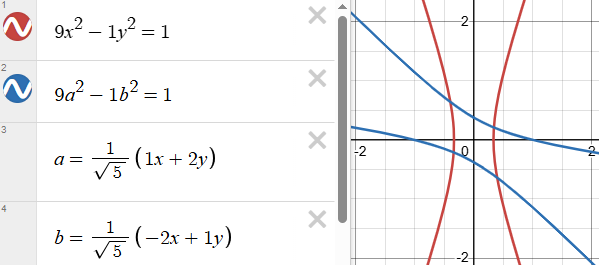
\includegraphics[width=0.8\textwidth]{P12.png}
\\$(x+y)(x+7y)=1$
\\asymtotes $x=-y$, $x=-7y$
\\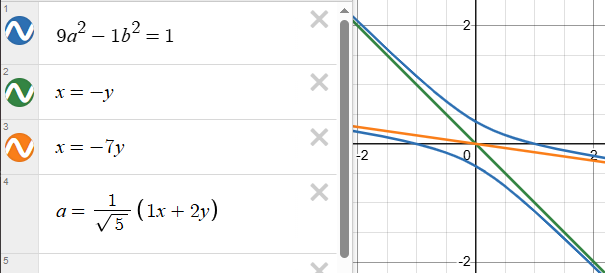
\includegraphics[width=0.8\textwidth]{P13.png}

\newpage\item Let $A$ be any real matrix and prove that
\begin{enumerate}[a.]
\item If $\bm{v}$ is an eigenvector of $AA^T$, then $\bm{v}\in{\rm range}(A)\cup{\rm null}(A^T)$ (look at the cases where the corresponding e-value is 0 or nonzero)
\\
\\let $A$ be an $m\times n$ matrix
\\$AA^Tv=\lambda v$
\\first case: $\lambda=0$
\\then $AA^Tv=0$
\\note $0=v^T(AA^Tv)=||A^Tv||^2$
\\so $A^Tv=0$
\\$v\in\textrm{ker}(A^T)$
\\second case: $\lambda\neq0$
\\$v=\frac{1}{\lambda}AA^Tv=A(\frac{1}{\lambda}A^Tv)$
\\so $v\in\textrm{range}(A)$
\\
\item If $\lambda$ is a nonzero eigenvalue of $AA^T$, then it is also an eigenvalue of $A^TA$
\\
\\let $\lambda\neq0$ and $v\neq0$, $AA^Tv=\lambda v$
\\set $u:=A^Tv$
\\if $u=0$, then $A^Tv=0$ would imply $AA^Tv=0$, contradicting $\lambda=0$, so $u\neq0$
\\$A^TAu=A^TA(A^Tv)=A^T(AA^Tv)=A^T(\lambda v)=\lambda(A^Tb)=\lambda u$
\\hence $u$ is an eigenvector of $A^TA$ with eigenvalue $\lambda$. 
\\therefore any nonzero eigenvalue of $AA^T$ is also an eigenvalue of $A^TA$

\end{enumerate}


\newpage\item Let $$A=\left[
\begin{array}{cc}
1 & 1\\
-1 & 1\\
1 & 2
\end{array}\right]$$

\begin{enumerate}[a.]
\item Find the singular value decomposition of $A$
\\
\\$A^TA=\left[\begin{array}{cc} 3 & 2 \\ 2 & 6 \end{array}\right]$
\\$\lambda_1=7$, $\lambda_2=2$
\\$\sigma_1=\sqrt{7}$, $\sigma_2=\sqrt{2}$
\\$v_1=\frac{1}{\sqrt{5}}\left[\begin{array}{c} 1 \\ 2 \end{array}\right]$, $v_2=\frac{1}{\sqrt{5}}\left[\begin{array}{c} -2 \\ 1 \end{array}\right]$
\\$V=\frac{1}{\sqrt{5}}\left[\begin{array}{cc} 1 & -2 \\ 2 & 1 \end{array}\right]$
\\let $u_i=\frac{1}{\sigma_i}Av_i$
\\$u_1=\frac{1}{\sqrt{35}}\left[\begin{array}{c} 3 \\ 1 \\ 5 \end{array}\right]$, $u_2=\frac{1}{\sqrt{10}}\left[\begin{array}{c} -1 \\ 3 \\ 0 \end{array}\right]$, 
\\choose $u_3=\frac{1}{\sqrt{14}}\left[\begin{array}{c} -3 \\ -1 \\ 2 \end{array}\right]$ orthonormal to $u_1$, $u_2$
\\$\Sigma = \left[\begin{array}{cc} \sqrt{7} & 0 \\ 0 & \sqrt{2} \\ 0 & 0 \end{array}\right]$
\\$A=U\Sigma V^T$
\\
\item Find the psuedo-inverse, $A^+$ and use it to find the vector in ${\rm range}~A$ that is closest to $\left[
\begin{array}{c}
1\\
2\\
3
\end{array}\right]$
\\
\\$A^+=V\Sigma^+U^T$
\\$\Sigma^+=\left[\begin{array}{ccc} \sqrt{7} & 0 & 0 \\ 0 & \sqrt{2} & 0 \end{array}\right]$
\\$A^+=\left[\begin{array}{ccc} \frac{2}{7} & -\frac{4}{7} & \frac{1}{7} \\ \frac{1}{14} & \frac{5}{14} & \frac{2}{7} \end{array}\right]$
\\for any $b\in\mathbb{R}^3$ the orthogonal projection of $b$ onto $\textrm{range}(A)$ is $P_{\textrm{range}A}b=AA^+b$
\\$\hat{x}=A^+b=\left[\begin{array}{c} -\frac{3}{7} \\ \frac{23}{14} \end{array}\right]$
\\$A\hat{x}=\left[\begin{array}{c} \frac{17}{14} \\ \frac{29}{14} \\ \frac{40}{14} \end{array}\right]$

\end{enumerate}


\newpage\item Find and sketch the image of the unit circle under the linear transformation $T:\mathbb{R}^2\rightarrow\mathbb{R}^2$ where
\begin{eqnarray*}
T\bm{e}_1&=&2\bm{e}_1+\bm{e}_2
\\ T\bm{e}_2&=&-3\bm{e}_1+6\bm{e}_2
\end{eqnarray*}
using the method from lecture 11-20
\\
\\$A=\left[\begin{array}{cc}2&-3\\1&6\end{array}\right]$
\\$y=A^{-1}x$, $y^Ty=1$, $x^T(AA^T)^{-1}x=1$
\\$AA^T=\left[\begin{array}{cc}13&-16\\-16&37\end{array}\right]$
\\$(AA^T)^{-1}=\frac{1}{225}\left[\begin{array}{cc}37&-16\\-16&13\end{array}\right]$
\\$\frac{37}{225}x_1^2+\frac{32}{225}x_1x_2+\frac{13}{225}x_2^2=1$
\\$\lambda_1=25$, $\lambda_2=5$
\\$u_1=\frac{1}{\sqrt{5}}\left[\begin{array}{c}-\frac{1}{2}\\1\end{array}\right]$
\\$u_2=\frac{1}{\sqrt{5}}\left[\begin{array}{c}2\\1\end{array}\right]$
\\$\sigma_1=3\sqrt{5}$, $\sigma_2=\sqrt{5}$
\\ellipse with semi axis lengths $\sigma_1$, $\sigma_2$ and principle directions are columns $u_1$, $u_2$
\\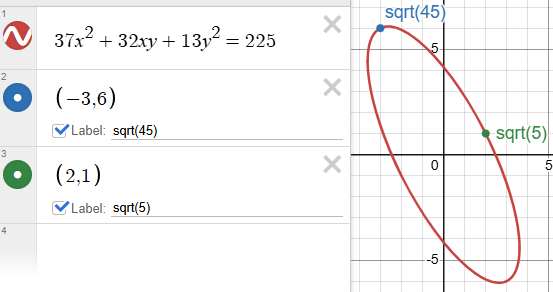
\includegraphics[width=0.8\textwidth]{P41.png}

\newpage\item Given $n\times n$ matrix $A$, define the trace of $A$ as
$${\rm tr(A)}=\sum_{i=1}^n A_{i,i}=\langle {\bm e}_1,A{\bm e}_1\rangle+\cdots +\langle {\bm e}_n,A{\bm e}_n\rangle$$

Now letting $A\in\mathbb{C}^{n\times n}$ have singular values of $\sigma_1,\cdots,\sigma_r$, show that  

$${\rm tr}(A^*A)=\sigma_1^2+\cdots+\sigma_r^2$$
\\
\\write SVD of $A$: $A=U\Sigma V^*$
\\where $U$, $V$ are unitary and $\Sigma=\textrm{diag}(\sigma_1,\ldots,\sigma_r,0,\ldots,0)$
\\$A^*A=(U\Sigma V^*)^*(U\Sigma V^*)=V\Sigma^*U^*U\Sigma V^*=V\Sigma^2V^*$
\\$U^*U=I$ and $\Sigma^*=\Sigma$
\\$\textrm{tr}(A^*A)=\textrm{tr}(V\Sigma^2V^*)=\textrm{tr}(V^*V\Sigma^2)=\textrm{tr}(\Sigma^2)$
\\$\Sigma^2=\textrm{diag}(\sigma_1^2,\ldots,\sigma_r^2,0,\ldots,0)$
\\so $\textrm{tr}(\Sigma^2)=\sigma_1^2+\ldots+\sigma_r^2$
\\Hence ${\rm tr}(A^*A)=\sigma_1^2+\cdots+\sigma_r^2$




\end{enumerate}

\end{document}

